% Luận văn — dựa trên Springer splncs04.bst cho tài liệu tham khảo
% Nội dung bám cấu trúc LNCS; document class report cho luận văn dài
%
% Compile: ./compile.sh
%
\documentclass[12pt,a4paper]{report}

\usepackage{fontspec}
\usepackage{polyglossia}
\setdefaultlanguage{vietnamese}
\setotherlanguage{english}
% Shared XeLaTeX font setup for Vietnamese manuscripts.
% TeX Gyre Termes is a Times-compatible font that ships with TeX Live / MacTeX,
% covers Vietnamese, and needs no MS-Office fonts -> builds on any machine.
% If you have "Times New Roman" installed and your venue requires it exactly,
% swap the line below for: \setmainfont{Times New Roman}[Ligatures=TeX]
\setmainfont{TeX Gyre Termes}[Ligatures=TeX]

\usepackage{graphicx}
\usepackage{booktabs}
\usepackage{amsmath}
\usepackage{hyperref}
\usepackage{geometry}
\geometry{margin=2.5cm}

\graphicspath{{../../results/ml_07_cross_method_comparison/}{../../results/ml_05_shap_explainability/}}

\title{%
  HỆ THỐNG PHÁT HIỆN XÂM NHẬP MẠNG\\
  SỬ DỤNG HỌC MÁY TRÊN APACHE SPARK\\
  VÀ TRIỂN KHAI PHÂN TÁN TRÊN THIẾT BỊ BIÊN
}
\author{%
  \begin{tabular}[t]{c}
    Nguyễn Vũ Thái\\[0.4em]
    {\small Sinh viên thực hiện}\\[0.2em]
    {\small Trường Đại học Giao thông Vận tải, Phân hiệu tại TP. Hồ Chí Minh}\\[0.2em]
    {\small \texttt{nvthai@utc2.edu.vn}}\\[1.2em]
    Bùi Văn Dũng\\[0.4em]
    {\small Giảng viên hướng dẫn}\\[0.2em]
    {\small Trường Đại học Công nghệ Thông tin, ĐHQG TP. Hồ Chí Minh}\\[0.2em]
    {\small \texttt{dungbv.17@grad.uit.edu.vn}}
  \end{tabular}%
}
\date{Năm 2026}

\begin{document}

\maketitle

\begin{abstract}
Luận văn nghiên cứu xây dựng hệ thống phát hiện xâm nhập mạng (IDS) nhị phân trên dataset CICIDS2017,
sử dụng Apache Spark ML với chín thuật toán phân loại và phương pháp ensemble.
So sánh bốn chiến lược giảm chiều: baseline, RF Importance, SHAP và PCA,
kèm đánh giá robustness, concept drift và kiểm định thống kê.
Triển khai edge realtime trên Raspberry Pi và cụm hai Jetson Nano với Kafka, PySpark và anomaly gate autoencoder.
Kết quả cho thấy [TODO: tóm tắt kết quả chính].
\end{abstract}

\tableofcontents
\listoffigures
\listoftables

\chapter{Giới thiệu}

\section{Bối cảnh và động lực}

% TODO: tấn công mạng, IDS, big data, edge computing

\section{Mục tiêu nghiên cứu}

\begin{enumerate}
  \item So sánh hiệu quả các phương pháp giảm chiều và lựa chọn đặc trưng trên Spark ML.
  \item Ứng dụng SHAP cho giải thích và lựa chọn đặc trưng IDS.
  \item Đánh giá robustness và concept drift trên CICIDS2017.
  \item Thiết kế và triển khai IDS phân tán trên thiết bị biên (Jetson Nano).
\end{enumerate}

\section{Phạm vi và giới hạn}

% TODO

\section{Cấu trúc luận văn}

Chương~2 trình bày cơ sở lý thuyết; Chương~3 mô tả phương pháp; Chương~4 báo cáo thí nghiệm ML; Chương~5 trình bày triển khai edge; Chương~6 kết luận.

\section{Công trình liên quan đã công bố}

Hai bài báo rút gọn từ luận văn:
\begin{itemize}
  \item FAIR'2026: so sánh giảm chiều và lựa chọn đặc trưng (Chương~3--4).
  \item SOICT 2026: triển khai phân tán trên Jetson Nano (Chương~5).
\end{itemize}

\chapter{Cơ sở lý thuyết}

\section{Phát hiện xâm nhập mạng}

% TODO: IDS, signature vs anomaly, CICIDS2017~\cite{sharafaldin2018toward}

\section{Học máy trên Apache Spark}

% TODO: Spark MLlib~\cite{zaharia2010spark}

\section{Lựa chọn đặc trưng và giảm chiều}

\subsection{Random Forest Feature Importance}
\subsection{SHAP --- SHapley Additive exPlanations~\cite{lundberg2017unified}}
\subsection{Phân tích thành phần chính (PCA)}

\section{Ensemble Learning}

% TODO: bagging, voting

\section{Edge computing và stream processing}

% TODO:~\cite{shi2016edge,kreps2011kafka}

\section{Phát hiện bất thường bằng Autoencoder}

% TODO:~\cite{chandola2009anomaly,hochreiter1997lstm}

\chapter{Phương pháp đề xuất}

\section{Tổng quan hệ thống}

Luận văn gồm hai pha: (1) huấn luyện và đánh giá offline trên PC với PySpark; (2) suy luận realtime trên edge qua Kafka.

\section{Chuẩn bị dữ liệu}

Script \texttt{data\_preparation.py}: gộp 8 file CSV CICIDS2017, làm sạch, nhãn nhị phân, chia 80/20, lưu Parquet.

\section{Pipeline huấn luyện Spark ML}

VectorAssembler $\rightarrow$ StandardScaler $\rightarrow$ Classifier / PCA.

\section{Bộ thí nghiệm (Exp 0--8)}

\begin{table}[htbp]
  \centering
  \caption{Mapping thí nghiệm và mục tiêu.}
  \begin{tabular}{cl}
    \toprule
    Exp & Mục tiêu \\
    \midrule
    0 & Baseline toàn bộ đặc trưng \\
    1 & RF Feature Importance (Top 20/30/40) \\
    2 & Grid Search + Cross-Validation \\
    3 & PCA ($k$ = 20/30/40) \\
    5 & SHAP explainability (XGBoost) \\
    6 & SHAP feature selection \\
    7 & So sánh chéo + drift + robustness \\
    8 & Autoencoder anomaly gate \\
    \bottomrule
  \end{tabular}
\end{table}

\section{Kiến trúc edge phân tán}

Ba chế độ: pipeline split, horizontal scaling, Spark cluster (xem \texttt{raspberry/JETSON\_DISTRIBUTED.md}).

\section{Chỉ số đánh giá}

Accuracy, Precision, Recall, F1, AUC-ROC, AUC-PR; thời gian huấn luyện/dự đoán; throughput và latency edge.

\chapter{Thí nghiệm và kết quả huấn luyện ML}

\section{Môi trường thí nghiệm}

% TODO: phần cứng PC, Java 17, PySpark 3.4.1

\section{Kết quả baseline (Exp 0)}

% TODO: bảng + hình từ results/ml_01_baseline/

\section{So sánh giảm chiều (Exp 1, 3, 6, 7)}

\begin{figure}[htbp]
  \centering
  \IfFileExists{../../results/ml_07_cross_method_comparison/f1_heatmap.png}{%
    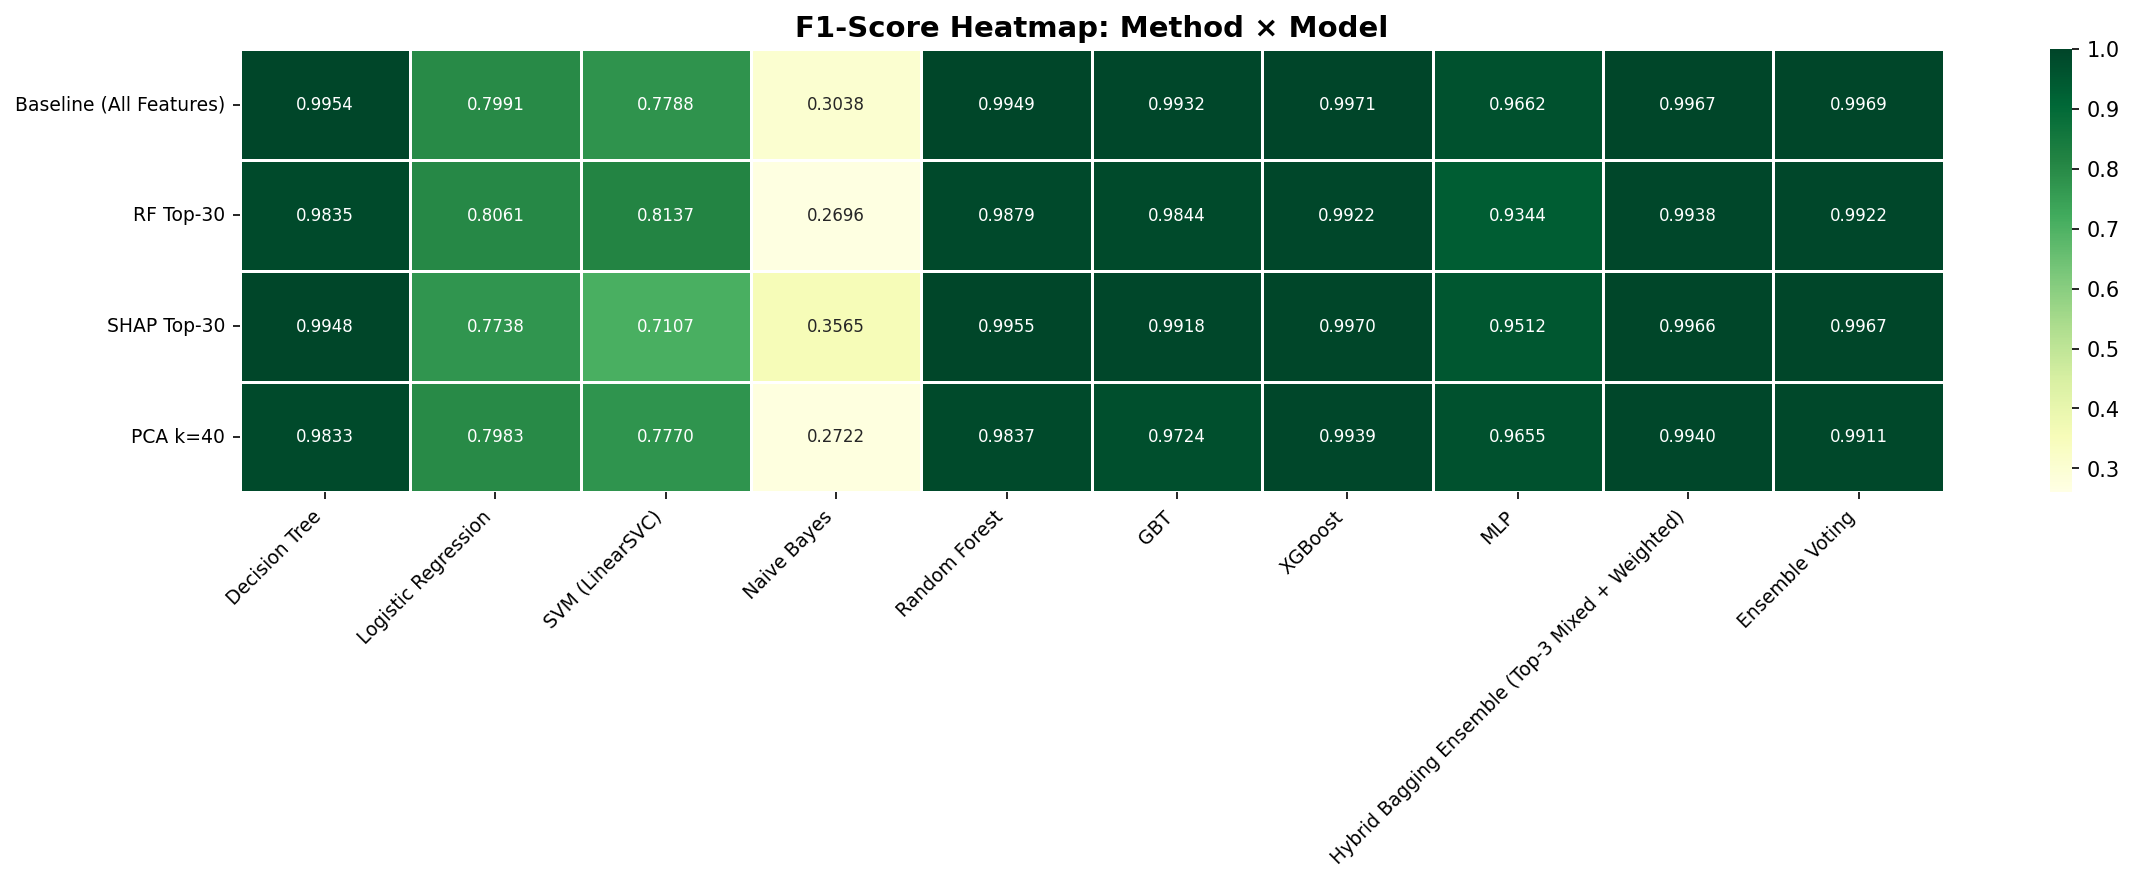
\includegraphics[width=0.95\textwidth]{f1_heatmap.png}%
  }{%
    \fbox{\parbox{0.9\textwidth}{\centering [Chạy thesis/collect\_results.sh]}}%
  }
  \caption{Heatmap F1 theo phương pháp và thuật toán.}
\end{figure}

\section{SHAP explainability (Exp 5)}

% TODO

\section{Grid Search (Exp 2)}

% TODO: best\_config.json

\section{Robustness, drift và kiểm định thống kê}

% TODO: drift\_simulation\_summary.csv

\section{Thảo luận}

% TODO: chọn DT / SHAP Top-30 cho edge

\chapter{Triển khai edge và đánh giá phân tán}

\section{Kiến trúc split deployment}

PC: Kafka, PostgreSQL, InfluxDB, Grafana. Edge: PySpark inference + tuỳ chọn anomaly gate.

\section{Xuất mô hình}

\texttt{raspberry/scripts/save\_model.py}, \texttt{ml\_08\_anomaly\_gate\_autoencoder.py}.

\section{Triển khai Raspberry Pi}

% TODO: latency, monitoring

\section{Triển khai phân tán trên 2 Jetson Nano}

\subsection{Chế độ pipeline split}
\subsection{Chế độ horizontal scaling}
\subsection{Chế độ Spark cluster}

\section{Kết quả benchmark edge}

% TODO: điền sau run_benchmarks.sh

\section{Giám sát và cảnh báo}

InfluxDB metrics theo \texttt{EDGE\_NODE\_ID}; alert Email/Slack/Telegram.

\section{Thảo luận}

So sánh với bài báo SOICT 2026; hạn chế phần cứng Nano 4GB.

\chapter{Kết luận và hướng phát triển}

\section{Tóm tắt kết quả}

% TODO

\section{Đóng góp chính}

\begin{enumerate}
  \item Pipeline Spark ML đánh giá toàn diện IDS trên CICIDS2017.
  \item So sánh RF, SHAP, PCA với drift và robustness.
  \item Hệ thống edge phân tán trên Jetson Nano với Kafka.
  \item Anomaly gate giảm tải suy luận Spark.
\end{enumerate}

\section{Hạn chế}

% TODO: dataset cũ, Jetson RAM, chưa thử nghiệm production

\section{Hướng phát triển}

TensorRT, federated learning, mở rộng RoEduNet, tích hợp SOC.

\section{Công trình công bố}

\begin{itemize}
  \item FAIR'2026 --- so sánh giảm chiều (Chương~3--4).
  \item SOICT 2026 --- edge phân tán Jetson Nano (Chương~5).
\end{itemize}


\bibliographystyle{../../papers/latex/splncs04}
\bibliography{references}

\end{document}
